\begin{figure}[t!]
\centering
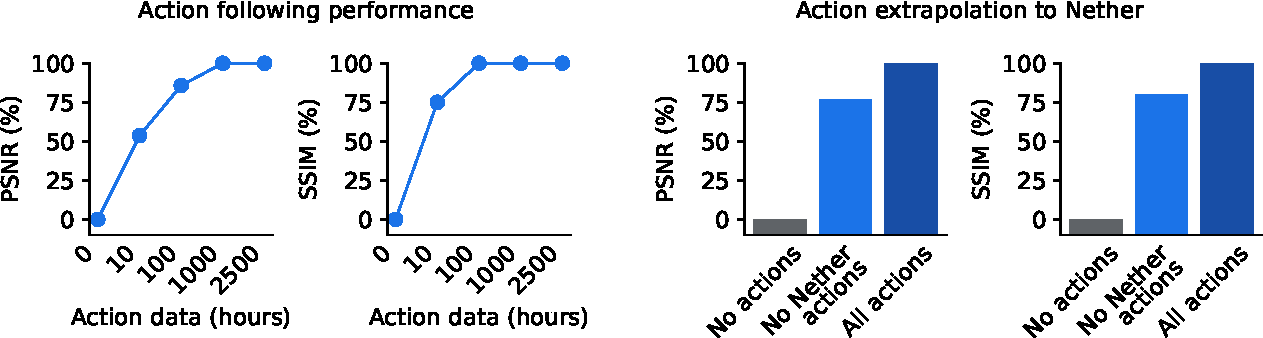
\includegraphics[width=\linewidth]{figures/actgen/actgen}
\caption{
Action generalization.
\textbf{(left)}
\method learns accurate action conditioning from 2500 hours of video with only 100 hours of paired actions.
It achieves over 80\% of the action-conditioned generation accuracy, normalized within the range of training without any actions and using all actions.
\textbf{(right)}
When learned with only actions of the Minecraft Overworld, the action conditioning generalizes to the Nether and End dimensions of the game that are only seen in unlabeled videos.
These environments are distinct from the Overworld in their textures, blocks, and items.
The results indicate that \method learns action conditioning from small amounts of action data that generalize broadly, paving the way toward learning simulators from diverse unlabeled web videos.
}
\label{fig:actgen}
\end{figure}